\chapter{Proposta} \label{cap:proposta}

Como visto no Capítulo 2, existe uma corrente dentro da Mineração de Opinião que vem desenvolvendo maneiras de explorar o conteúdo digital gerado pela nossa sociedade todos os dias em redes sociais, através de técnicas utilizando Processamento de Linguagem Natural e \textit{Machine Learning}, principalmente. Com este fato surge a oportunidade de explorar novas ferramentas na
solução de problemas que envolvem pesquisas de opinião de forma geral.
Neste trabalho propõem-se um \textit{framework} que torna possível fazer pesquisas de opiniões em língua portuguesa sobre qualquer tema que seja rastreável a partir de uma \textit{hashtag} no Twitter.
Para tal é necessário que o framework criado seja capaz de:

\begin{enumerate}
	\item Coletar \textit{tweets} escritos em língua portuguesa que contenham uma determinada {hashtag};
	\item Armazenar as mensagens em uma base de dados;
	\item Classificar as mensagens de acordo com a polaridade: negativo, neutro e positivo;
	\item Extrair \textit{insights} que auxiliem a tomada de decisão a partir da massa de dados classificada;
\end{enumerate}

\section{Coleta de dados}
A plataforma do Twitter conecta aplicações e sites com seus dados através de diversos serviços. Para este trabalho, a principal fonte de dados será sua API REST, que possui uma excelente documentação disponível em \cite{twitterapidocs}. Através dela é possível acessar informações de usuários e \textit{tweets}, assim como escrever novas mensagens. Além disso, a API conta com um mecanismo de busca poderoso, que será fundamental para a coleta de dados. Os dados são entregues no formato \ac{JSON}.

\subsection{Autenticação}

Para que ter acesso à API antes é necessário possuir uma conta no Twitter e criar uma \textit{app} - através do próprio site \cite{twitterapp} - que utilizará o protocolo de autenticação OAuth\cite{oauth} para acessar os dados do Twitter se passando pelo usuário em questão. O objetivo do protocolo OAuth é permitir que uma aplicação se autentique em outra "em nome de um usuário". A aplicação pede permissão de acesso ao usuário, que possui a escolha de conceder permissão ou não. Um ponto importante: o usuário não precisa informar a sua senha para se autenticar, portanto a permissão continua vigente caso a senha do usuário se altere, o que permite que a aplicação não precise de manutenção neste caso, tornando-a mais resiliente. A autenticação por meio do OAuth necessita de três passos:

\begin{enumerate}
	\item Aplicação cliente obtém chave de autenticação;
	\item Usuário autoriza aplicação cliente na aplicação servidora;
	\item Aplicação cliente troca a chave de autenticação pela chave de acesso;
\end{enumerate}

Após o processo de criação da app, é criado um token de acesso que deve ser utilizado pelo sistema que deseja se autenticar no Twitter em nome de um usuário. Este token deve ser incorporado em cada requisição à API do Twitter para autenticar a mesma e dizer ao Twitter qual é a fonte do acesso.

\subsection{Limite de requisições}
A fim de evitar grande concentração de requisições em seus serviços, o Twitter implementa um limitador em sua API \cite{twitterrequestlimit2016}. São permitidas até 180 requisições por janela, que dura 15 minutos. Caso o limite seja ultrapassado, o serviço passa a retornar um erro na resposta, até que a "janela" de 15 minutos se renove.
A partir da versão 1.1 da API, novos cabeçalhos HTTP são retornados provendo feedback sobre os limites para requisição. Este recurso permite que o código consiga entender em que momento da janela se encontra, quantos requisições ainda podem ser feitas neste período de tempo e quanto é necessário esperar para poder fazer novas requisições. Os cabeçalhos em questão são:

\begin{itemize}
	\item X-Rate-Limit-Limit: A faixa limite para o requisição em questão;
	\item X-Rate-Limit-Remaining: O número de requisições que ainda restam para a janela de 15 minutos;
	\item X-Rate-Limit-Reset: O tempo restante dentro da janela de requisições atual, dado em segundos.
\end{itemize}

\subsection{Arquitetura}

Neste trabalho, como o objetivo é coletar \textit{tweets} postados sobre uma \textit{hashtag} em tempo real para utilizá-los como matéria-prima para análise de sentimento, é muito importante aproveitar ao máximo cada janela de requisições. Por este motivo, o sistema que coleta os dados da API do Twitter foi inspirado no modelo produtor-consumidor\cite{jeffay1993real} visando minimizar as perdas que podem acontecer em momentos de pico - como o começo ou clímax do evento, onde o volume de mensagens é maior, como veremos a frente no Capítulo 4 - e se necessário, escalar de forma simples durante os mesmos. 

\subsubsection{Produtor-consumidor}

O problema descreve dois processos, o produtor e o consumidor, que compartilham um recurso em comum usado como uma fila - um tipo particular de coleção de dados onde a primeira a entidade a entrar é a primeira a sair ou \ac{FIFO} . A função do produtor é gerar trabalho a ser executado pelo consumidor. O volume de trabalho gerado e executado pelo sistema é controlado pela fila, que armazena as entidades ou "tarefas" a serem executadas. Essa abordagem permite que o sistema escale apenas até a sua capacidade, visto que a fila possui um tamanho fixo que caso seja ultrapassado, pode simplesmente descartar as mensagens adicionadas após este momento. Outra característica importante é a escalabilidade. Conforme os processos produtor e consumidor evoluem, surge a necessidade de aumentar a quantidade de produtores ou consumidores de forma independente.

Neste trabalho, para explorar o potencial máximo da janela de requisições foi criado um processo produtor que envia para a fila mensagens para que consumidor acesse à API do Twitter de forma que sejam feitos sempre as 180 requisições que são permitidas no intervalo de 15 minutos. Assim a responsabilidade de cada processo fica bem definida - o primeiro responde pelo volume de requisições e o segundo por realizar a requisição e entender a resposta. Para definir qual intervalo de tempo deveria ser usado para que o produtor envie mensagens à fila, foi feita uma conta simples:

$$ \frac{180}{15} = 12 \textit{ requests}_{/minuto} $$

Logo, o produtor precisa adicionar uma mensagem na fila a cada 5 segundos, para que o limite de 180 requisições seja respeitado.

\begin{figure}[H]
	\centering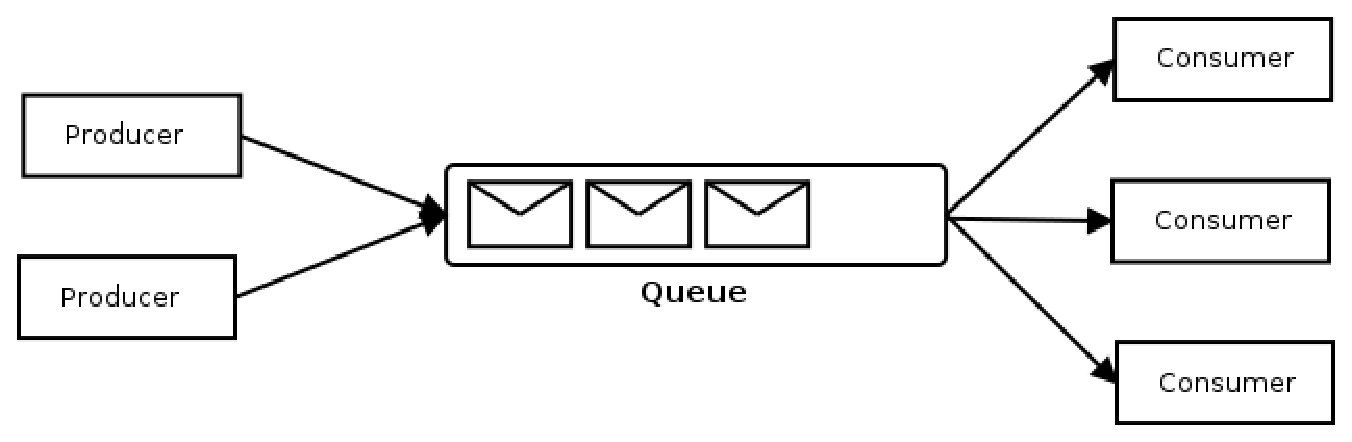
\epsfig{file=figuras/competing-consumers.eps, width=15cm}
	\caption{Exemplo de arquitetura produtor-consumidor. Fonte: Apache ActiveMQ( http://activemq.apache.org/clustering.html)}
	\label{time}
\end{figure}


\subsection{Busca}
Dentre os principais serviços da API do Twitter está a busca. Com ela, é possível consultar de diversas formas os principais \textit{tweets} ou mais recentes. Dentro de sua documentação, existe um guia completo de como utilizar a API  para extrair os resultados desejados \cite{twittersearchapi} das mais diversas formas. 

\subsubsection{Parâmetros adicionais}

Como abordado acima, a API possui diversos parâmetros que podem ser usados para que o usuário chegue a um conjunto de dados mais próximo da sua necessidade:

\begin{itemize}
	\item \textit{\textbf{result\_type}}: permite escolher se o resultado da busca será representado pelos \textit{tweets} mais populares (\textit{popular}) ou mais recentes (\textit{recent});
	\item \textit{\textbf{geocode}}: permite buscar por uma determinada latitude, longitude e raio, respectivamente, separando-os por vírgula. ex: geocode=-22.912214,-43.230182,1km;
	\item \textit{\textbf{lang}}: restringe os \textit{tweets} buscados a um idioma específico. ex: lang=pt;
	\item \textit{\textbf{since\_id }},  \textit{\textbf{max\_id }}, \textit{\textbf{count}} e \textit{\textbf{until}}: possibilita iterar através dos resultados quando existe um grande números de \textit{tweets} a percorrer. De acordo com a concorrência e o volume, esta tarefa pode ficar mais complicada. Uma leitura recomendada se encontra em \cite{workingwithtimelimes}.
\end{itemize}

Como o objetivo deste trabalho é coletar novos \textit{tweets} conforme eles vão sendo postados, foi necessário utilizar apenas dois parâmetros da API de busca: \textit{count} e \textit{since id}. O primeiro tem o objetivo de garantir o número máximo de registros retornados pela API e o segundo define de onde se pretende partir para buscar novos \textit{tweets}, evitando que mensagens repetidas sejam coletadas.

\url{https://api.twitter.com/1.1/search/tweets.json?q=#oscars2016&count=100&since_id=123456789}

Neste caso, a API retornará os 100 \textit{tweets} publicados desde o \textit{tweet} com identificador (\textit{id}) "123456789".

\todo{Diagrama de sequência ou atividades sobre como esta parte do código funciona}

\subsubsection{O problema com a detecção automática de idioma do Twitter}

O escopo deste trabalho determina que o objeto de estudo são apenas mensagens escritas em língua portuguesa. Como forma de obter somente \textit{tweets} escritos em língua portuguesa é preciso utilizar o parâmetro \textit{lang}, por exemplo:

\url{https://api.twitter.com/1.1/search/tweets.json?q=#oscars2016&lang=pt&result_type=recent}

Porém, realizando alguns testes na API do Twitter, foi detectado que ao submeter algum \textit{tweet}, alguma rotina dentro do próprio Twitter atribui um idioma à mensagem automaticamente. Nos testes conduzidos durante este trabalho foi identificado que em mensagens curtas - algo recorrente no Twitter - o algoritmo apresenta resultados aquém do esperado na identificação do idioma, visto que as poucas palavras contidas na mensagem podem ser comuns a mais de um idioma. Por conta disso foi decidido que o filtro de idioma não seria utilizado. Esta decisão pode mudar de acordo com o evento monitorado ou com o escopo do estudo.

\subsubsection{Escalando de forma horizontal}

Por uma questão de desenho da API de busca, cada requisição é capaz de trazer no máximo 100 \textit{tweets}, o que nos dá ao total uma carga máxima de até 1200 novos \textit{tweets} por minuto. Para as análises feitas durante este trabalho este número se mostrou mais do que suficiente. Como dito anteriormente, se fosse necessário escalar este sistema para monitorar um evento maior, seria necessário apenas obter um saldo maior de requisições junto a API do Twitter - adicionando mais tokens de usuário e criando uma espécie de "rodízio" de autenticações, por exemplo - e escalar o número de consumidores do processo de acordo com a demanda. Uma boa maneira de detectar se isso seria necessário é acompanhar quantos \textit{tweets} novos são coletados a cada requisição. Como utilizamos o \textit{id} do último \textit{tweet} capturado como referência para os novos, se a cada requisição o número de novos \textit{tweets} com grande frequência coincidir com o limite da API, temos um indício de que o volume de novas mensagens no Twitter está excedendo a capacidade do sistema de coletá-las e que o excedente está sendo perdido.

\section{Armazenamento}
A resposta da API de Busca é dada no formato JSON e cada objeto - que corresponde a cada \textit{tweet} - segue o seguinte formato e conta com diversas informações sobre o mesmo: 

\begin{lstlisting}[style=json, frame=single]
{
	"_id" : "56d388096861353c1b061fe2",
	"contributors" : null,
	"truncated" : false,
	"text" : "Leonardo DiCaprio com o #oscars eh igual a Katy Perry com o Grammy #OscarsNaTNT",
	"is_quote_status" : false,
	"in_reply_to_status_id" : null,
	"id" : 704091511902834688,
	"favorite_count" : 0,
	"source" : "<a href=\"http://twitter.com/download/android\" rel=\"nofollow\">Twitter for Android</a>",
	"created_at_datetime" : ISODate("2016-02-28T20:51:12.000Z"),
	"retweeted" : false,
	"coordinates" : null,
	"created_at_timestamp" : 1456714272.0000000000000000,
	"entities" : {
		"symbols" : [],
		"user_mentions" : [],
		"hashtags" : [{
			"indices" : [ 24, 31 ],
			"text" : "oscars"
		}, 
		{
			"indices" : [ 66, 78],
			"text" : "OscarsNaTNT"
		}],
		"urls" : []
	},
	"in_reply_to_screen_name" : null,
	"id_str" : "704091511902834688",
	"retweet_count" : 0,
	"in_reply_to_user_id" : null,
	"favorited" : false,
	"user" : {
		"follow_request_sent" : false,
		"has_extended_profile" : true,
		"profile_use_background_image" : false,
		"id" : 2786117482,
		"verified" : false,
		"profile_text_color" : "000000",
		"profile_image_url_https" : "https://pbs.twimg.com/profile_images/700450356141158404/xA-mRqp7_normal.jpg",
		"profile_sidebar_fill_color" : "000000",
		"is_translator" : false,
		"entities" : {
			"description" : {
			"urls" : []
			}
		},
		"followers_count" : 156,
		"protected" : false,
		"location" : "Um lugarzinho no fim do mundo",
		"default_profile_image" : false,
		"id_str" : "2786117482",
		"lang" : "pt",
		"utc_offset" : -28800,
		"statuses_count" : 6171,
		"description" : "Uuuumm ta estilosa!",
		"friends_count" : 192,
		"profile_background_image_url_https" : "https://abs.twimg.com/images/themes/theme1/bg.png",
		"profile_link_color" : "9266CC",
		"profile_image_url" : "http://pbs.twimg.com/profile_images/700450356141158404/xA-mRqp7_normal.jpg",
		"notifications" : false,
		"geo_enabled" : false,
		"profile_background_color" : "000000",
		"profile_banner_url" : "https://pbs.twimg.com/profile_banners/2786117482/1456444936",
		"profile_background_image_url" : "http://abs.twimg.com/images/themes/theme1/bg.png",
		"name" : "Padeira Estilosa",
		"is_translation_enabled" : false,
		"profile_background_tile" : false,
		"favourites_count" : 6095,
		"screen_name" : "naycordeir",
		"url" : null,
		"created_at" : "Fri Sep 26 18:43:47 +0000 2014",
		"contributors_enabled" : false,
		"time_zone" : "Pacific Time (US & Canada)",
		"profile_sidebar_border_color" : "000000",
		"default_profile" : false,
		"following" : false,
		"listed_count" : 1
	},
	"geo" : null,
	"in_reply_to_user_id_str" : null,
	"lang" : "pt",
	"created_at" : "Sun Feb 28 23:51:12 +0000 2016",
	"metadata" : {
		"iso_language_code" : "pt",
		"result_type" : "recent"
	},
	"in_reply_to_status_id_str" : null,
	"place" : null
}
\end{lstlisting}

Dentro desta resposta, existem diversos dados que podem ser úteis para análises em cima dos \textit{tweets} e armazená-los é extremamente valioso.

\subsection{Banco de dados orientado a documento}

Existem diversas soluções de banco de dados disponíveis no mercado. Nos últimos anos, uma delas se tornou especialmente popular\cite{bhuvan2015technical}: os bancos de dados orientado a documento. Tais bancos de dado são uma das principais categorias de bancos conhecidos NoSQL (\textit{Non Structure Query Language}) que consiste em organizar os dados de forma "não-relacional", através de documentos, gráficos, chave-valores e colunas. Bancos NoSQL são conhecidos pela facilidade de modelagem e desenvolvimento, alto desempenho de leitura e escrita, alta disponibilidade e resiliência. Isso não significa que bancos SQL são obsoletos ou piores, porém existem aplicações claras onde cada um desempenha um melhor papel. Podemos apontar algumas comparações, como por exemplo:

\begin{table}[H]
	\label{tabela-sql-nosql}
	\begin{tabular}{|m{2.5cm}|m{6cm}|m{6cm}|}
		 \hline	
		& Banco de dados relacional                                                                                                                                                                                                                            & Banco de dados NoSQL                                                                                                                                                                                                                                                                                                                \\ \hline 
		Modelagem   & O modelo relacional normaliza dados em estruturas tabulares conhecidas como tabelas, que consistem em linhas e colunas. Um schema define estritamente as tabelas, colunas, índices, relações entre tabelas e outros elementos do banco de dados.     & Bancos de dados não relacionais (NoSQL) normalmente não aplicam um schema. Geralmente, uma chave de partição é usada para recuperar valores, conjuntos de colunas ou documentos semiestruturados JSON, XML ou outros que contenham atributos de itens relacionados.                                                                  \\ \hline 
		Desempenho  & O desempenho normalmente depende do subsistema do disco. A otimização de consultas, índices e estrutura de tabela é necessária para alcançar máximo desempenho.                                                                                      & Desempenho geralmente é uma função do tamanho do cluster do hardware subjacente, da latência de rede e da aplicação que faz a chamada.  \\ \hline 
		Escala      & Mais fácil de aumentar a escala "verticalmente" com hardware mais rápido.,Outros investimentos são necessários para tabelas relacionais para abranger um sistema distribuído.                                                                        & Projetado para aumentar a escala "horizontalmente" usando clusters distribuídos de hardware de baixo custo para aumentar a transferência sem aumentar a latência.                                \\ \hline 
		APIs & As solicitações para armazenar e recuperar dados são comunicadas usando consultas compatíveis com structured query language (SQL). Essas consultas são analisadas e executadas por sistemas de gerenciamento de bancos de dados relacionais (RDBMS). & APIs baseadas em objetos permitem que desenvolvedores de aplicações armazenem e restaurem facilmente estruturas de dados na memória. As chaves de partição permitem que os aplicativos procurem pares de chave-valor, conjuntos de colunas ou documentos semiestruturados contendo objetos e atributos de aplicativos serializados. \\ \hline 
	\end{tabular}
		\caption{Comparação entre bancos SQL e NoSQL}
\end{table}

\subsection{Opções disponíveis}
O movimento de adoção de bancos \textit{NoSQL} está bastante enraizada no mundo \textit{open source}. Alguns projetos como Voldemort\cite{voldemortproject}, MongoDB\cite{mongodb}, Tokyo Cabinet\cite{tokyocabinet} e CouchDB\cite{couchdb}. Apesar de uma grande quantidade de opções \textit{open source}, o movimento ganhou muita força com a publicação de duas publicações sobre implementações proprietárias: o Google BigTable\cite{chang2008bigtable} e o Amazon Dynamo\cite{decandia2007dynamo}. Para este trabalho, a opção escolhida foi o MongoDB, altamente popular na comunidade \textit{open source} e com bastante material disponível com melhores práticas de criação, manutenção e configuração.

\subsection{Armazenando \textit{tweets}}
O objetivo deste trabalho é monitorar eventos através das \textit{hashtags}. E para cada uma delas é criada uma coleção - nome dado a um conjunto de documentos - dentro do banco de dados. O nome da coleção é dado pela \textit{hashtag} monitorada, como por exemplo \mbox{\#Oscars2016}.

No momento onde o processo consumidor - responsável por fazer requisições na API e lidar com o retorno - é ligado ocorre a criação da coleção, caso a mesma não exista, e dentro dela começam a ser armazenados os \textit{tweets} retornados pela API, obedecendo ao mesmo formato enviado pelo Twitter. Antes do armazenamento no banco alguns campos a mais são adicionados, mas vamos entrar neste detalhe apenas na seção sobre Classificação.

\section{Classificação}
\begin{itemize}
	\item Aplicar técnicas de normalização no texto. As mesmas devem ser específicas para a língua portuguesa;
	\item Construir base de palavras e termos classificados utilizadas como insumo para o modelo matemático;
	\item Preparar uma massa de treino para validar o modelo matemático antes da execução;
	\item Calibragem do algoritmo
	\item Salvar infos sobre a classificação dentro do documento
\end{itemize}

Durante o estudo foram utilizadas algumas ferramentas que auxiliaram o processo de classificação. A principal delas foi a \ac{NLTK} \cite{nltk_docs}, uma biblioteca em Python construída como suíte de soluções para trabalhar com linguagem natural. O NLTK conta com mais de 50 corpus linguísticos - conjunto de registros orais de uma determinada língua que servem como base para análises - além de diversas ferramentas para classificação, tokenização, marcação e análise de texto. Seguindo uma documentação específica para aplicação em língua portuguesa\cite{nltk_portuguese}, foram utilizados os seguintes corpus do NLTK durante este trabalho:

\begin{itemize}
	\item Floresta Sintá(c)tica Corpus versão 7.4: uma colaboração entre a Linguateca\cite{linguateca} e o projecto VISL\cite{visl}. Contém textos em português (do Brasil e de Portugal) analisados automaticamente pelo analisador sintáctico PALAVRAS (Bick 2000) e revistos por linguistas.
	\item Mac Morpho: Palavras extraídas a partir de textos do jornal Folha de São Paulo 
	\item Machado: Obra completa do escritor Machado de Assis
\end{itemize}

O processo de classificação é a alma deste projeto. É ele que determina qual sentimento será possível extrair de um \textit{tweet} através conteúdo altamente resumido do mesmo. Durante o estudo e aperfeiçoamento deste processo foram utilizadas algumas técnicas que visam:

\begin{itemize}
	\item Excluir do texto termos que são inúteis semanticamente, como por exemplo conjunções, preposições e marcações de usuários, conhecidas como \textit{mentions};
	\item Diminuir a variabilidade de aplicações para uma palavra dentro da língua portuguesa. ex: aplicação de gênero, plurais e singulares, conjugações verbais, entre outras;
	\item Treinar o algoritmo de classificação com uma base de palavras pertences ao mesmo universo e temática do estudo, permitindo que o algoritmo previamente conheça o contexto e força que alguns termos vão exercer sobre o texto.
\end{itemize}

\subsection{\textit{Stemming}}
\todo{Falar sobre Stemming}

\subsection{\textit{Stopwords}}

A composição de um \textit{tweet} por muitas vezes possui palavras que são semanticamente nulas ou até mesmo nocivas para o nosso algoritmo de classificação. Por conta disso, uma das primeiras técnicas aplicadas em um texto antes da classificação consiste em conduzir uma normalização nos elementos contidos em uma sentença.

Palavras que não possuem valor semântico para uma sentença são conhecidas como "palavras vazias" ou \textit{stopwords}. o NLTK possui um vasto dicionário de palavras vazias graças aos corpus de língua portuguesas adicionados à ele anteriormente. Com base neste dicionários, é possível excluir palavras vazias da seguinte forma:

\begin{lstlisting}[style=python, frame=single]
In[1]: text = "Veja a lista completa dos vencedores do Oscar 2016"
In[2]: [i for i in text.split() if i not in stopwords.words("portuguese")]

Out[1]:["Veja", "lista", "completa", "vencedores", "Oscar", "2016"]
\end{lstlisting}

Além disso, foi necessário adicionar inteligência ao nosso normalizador para também excluir palavras vazias específicas para \textit{tweets}, como por exemplo as \textit{hashtags}, menções a outros usuários - as \textit{mentions} - e \textit{links} para outras páginas, vídeos ou imagens.

\begin{lstlisting}[style=python, frame=single]
In[1]: TWITTER_STOPWORDS = ["@","RT","http"]
In[2]: def clean_stopwords(self, text):
  # Cleaning portuguese stopwords
  splitted = [i for i in text.split() if i not in stopwords.words("portuguese")]
  cleaned_splitted = []

  # Cleaning twitter stopwords
  for word in splitted:
    cleaned_splitted.append(word)

    for twitter_stopword in TWITTER_STOPWORDS:
      if word.startswith(twitter_stopword):
        cleaned_splitted.remove(word)

  return " ".join(cleaned_splitted)

In[2]: text = "@tntbr esta comecando agora a transmissao ao vivo do #Oscars2016 http://bit.ly/oscarstnt"
In[3]: clean_stopwords(text)

Out[1]: "esta comecando agora transmissao vivo"

\end{lstlisting}



\subsection{Construção da base de palavras e termos}
A construção da base de dados foi feita com o intuito de melhor expressar um sentimento de uma palavra ou texto, para a utilização do algoritmo. Para isso a base foi dividida em dois arquivos, positivos e negativos. Além dessa divisão foi utilizada outas bases criadas como: Re-li(referencia), SentiLex-PT \cite{marioj.silvapaulacarvalholuissarmento2012}, base da puc \cite{freitas2013construccao}, emoticons \cite{alexanderhogenboomdaniellabalflaviusfrasincarmalissabalfranciskadejonguzaykaymak}. Todas usando a língua portuguesa ou um linguajar universal, no caso dos emoticons e já estarem polarizadas. Essas bases têm em comum é serem feitas apenas de palavras, então ficou-se a dúvida de como a classificação funcionaria posteriormente quando aplicadas a um texto que as palavras podem não estar no mesmo contexto. Ex: "O flamengo jogou muito mal, mas fico feliz pela vitória", onde tem a palavra mal que já dá um tom negativo a frase , porém ao terminar de ler a frase encontrasse as palavras feliz e vitória que tem um contexto positivo.
Com essas bases já citadas foi compreendida a necessidade de uma base mais específica para o linguajar utilizado na internet, constituído de  
gírias, abreviação e até erros de português, para isso foi criada uma base utilizando dados pegos do twitter a partir da marcação hashtagoscar2016.

\subsection{Massa de Treino}

\subsection{Classificação}

\subsection{Algoritmo}

\subsection{Análises e \textit{insights}}